% a slightly adapted Copy of https://tex.stackexchange.com/questions/181081/clickable-chapters-on-the-right-side-of-each-page
% The credit goes to Gonzalo Medina, I only made slight changes (Converted to landscape and made Tabs nameable)

% ANOTHER IMPORTANT NOTE: The Boxlayout with Titles was copied from here: https://www.overleaf.com/articles/130-cheat-sheet/ntwtkmpxmgrp
% The Credit goes to Drew Ulick

\documentclass[8pt]{extarticle}
% Article
% \documentclass[9pt]{extarticle}
\usepackage[landscape, left=0.50cm, top=0.75cm, right=0.50cm, bottom=1.0cm, footskip=15pt]{geometry}
\usepackage{background}
\usepackage{etoolbox}
\usepackage{graphicx}
\usepackage{totcount}
\usepackage{lipsum}
\usepackage{hyperref}
\usepackage{amsmath}
\usepackage{amssymb}
\usepackage{physics}

%\usepackage{sectsty}
%\subsectionfont{\normalfont\large\itshape\underline}


% Tables
\usepackage{tabularx, multirow}
\usepackage{booktabs}
\renewcommand*{\arraystretch}{2}

% commands
\newcommand{\R}{{\mathbb R}}
\newcommand{\C}{{\mathbb C}}
\newcommand{\X}{{\mathcal X}}
\newcommand{\ra}{{\rightarrow}}
\newcommand{\Ra}{{\Rightarrow}}
% Math helper stuff
\def\limn{\lim_{n\to \infty}}
\def\limxo{\lim_{x\to 0}}
\def\limxi{\lim_{x\to\infty}}
\def\limxn{\lim_{x\to-\infty}}
\def\sumk{\sum_{k=1}^\infty}
\def\sumn{\sum_{n=0}^\infty}
\def\R{\mathbf{R}}
\def\dx{\text{ d}x}


% color text
\usepackage{xcolor}
\usepackage{tcolorbox}
% image directory
\graphicspath{ {./assets/} }

% For accessing arrays
\usepackage{etoolbox}


% for emumerating
\usepackage{enumitem}

% for color coding
\usetikzlibrary{backgrounds}

% for light font +C
\usepackage{color}
\definecolor{light}{rgb}{0.5, 0.5, 0.5}
\def\light#1{{\color{light}#1}}

% for multicolumn
\usepackage{multicol}
\setlength{\columnseprule}{0.4pt}

% to have access to the total number of sections
%\regtotcounter{section}

% every section starts on a new page
\pretocmd{\section}{\clearpage}{}{}

% auxiliary lengths for the height of the frame and the width of each tab
\newlength\mylen
\newlength\mylena

% style for the section tabs
\tikzset{
tab/.style={
  text width=\mylena,
  draw=gray,
  thick,
  rectangle,
  rounded corners=12pt,
  align=center,
  text width=53pt,
  inner sep=0pt,
  fill=gray!20,
  font=\sffamily\LARGE
  }
}
% style for the current section tab
\tikzset{selectedtab/.style={tab,color=white,fill=gray!90}}

% the page number is showed in the background material
%\pagestyle{empty}


% define the tab names
\newcounter{mylistcounter}

\def\saveitem#1{%
\stepcounter{mylistcounter}%
\expandafter\def\csname mylist\themylistcounter\endcsname{#1}}

\forcsvlist{\saveitem}{%
  Differential Equ.,
  $\R^n$ Differentials,
  $\R^n$ Integrals,
  Other
}%
\renewcommand*{\arraystretch}{2}
\allowdisplaybreaks

\def\getnthelement#1{\csname mylist#1\endcsname}

% the main part; as background material we place the border, 
% the section (current and other) tabs and the page number
\backgroundsetup{
scale=1,
color=black,
angle=0,
opacity=1,
contents={}
}

% define box
\tikzstyle{fancytitle} =[fill=black, text=white, font=\bfseries]
\begin{document}
\setlength{\columnseprule}{0.4pt}
\pagenumbering{arabic}
\begin{multicols*}{3}


  \section{Differential Equations}
  \hypertarget{sec:0}{}


  %------------ Linear ODE's ---------------
  \subsection{Linear ODE's}
  A differential equation is said to be linear if $F$
  can be written as a linear combination of the derivatives of $y$:
  \begin{align*}
    b(x) = \sum_{i = 0}^{n} a_i(x) \cdot y^{(i)}
  \end{align*}
  where $a_i(x)$ and $b(x)$ are continuous functions. Why is
  this called linear?
  \begin{align*}
    D                      & = \frac{d^{(k)}}{dx^k} + a_{k-1} \frac{d^{(k-1)}}{dx^{k-1}} + \dots + a_0 \\
    D(\alpha f + \beta g)  & = \alpha D(f) + \beta D(g)                                                \\
    Df_1 = b_1, Df_2 = b_2 & \Rightarrow D(f_1 + f_2) = b_1 + b_2
  \end{align*}

  %------------ Solution Space ---------------
  \subsection{Solution Space}
  Let $I \subset \R$ be an open interval
  and $k \geq 1$ an integer, and let
  \begin{align*}
    y^{(k)} + a_{k-1}y^{(k-1)} + \dots + a_1 y' + a_0 y = 0
  \end{align*}
  be a linear ODE over $I$ with continuous coefficients.
  \begin{enumerate}[label=(\arabic*)]
    \item The set $S$ of $k$-times differentiable solutions
          $f:I \ra \C$ of the equation is a complex
          vector space wich is a subspace of the space of complex valued
          funcitons on $I$. (Analogous for real numbers, if all
          $a_i$ are real valued)
    \item The dimension of $S$ is $k$ and for any choice of $x_0 \in I$
          and any $(y_0, \dots, y_{k-1}) \in \C^k$ there
          exists a unique $f$ such that
          \begin{align*}
            f(x_0) = y_0, f'(x_0) = y_1, \dots, f^{(k-1)}(x_0) = y_{k-1}
          \end{align*}
          (Analogous for real numbers, if all $a_i$ are real)
    \item For an arbitrary $b$ the solution set is
          $S_b = \{f + f_p \;|\; f \in S_0\}$ where $f_p$ is a "particular"
          solution.
    \item For any initial condition there is a unique solution.
  \end{enumerate}
  \subsection{Solving linear ODE's of order $1$}
$y' + ay = b.$ Here $a, b$ are constant functions.
\begin{tcolorbox}[colback=blue!5!white,colframe=blue!75!black]
  \begin{enumerate}[label=(\arabic*)]
    \item Find solutions of the corresponding homogenous equation
          $y' + ay = 0$. Note that if $f$ is a solution so is
          $z \cdot f \quad \forall z \in \C$.
          Example:
          \begin{align*}
            y' + ay      & = 0                                                \\
            y'           & = -ay                                              \\
            \frac{y'}{y} & = -a                                               \\
            ln(y)        & = - \int a \light{+C} = -A \light{+C}              \\
            y            & = e^{-A \light{+C}} = z \cdot e^{-A}\quad z \in \C
          \end{align*}
    \item Find a particular solution $f_p: I \ra \C$
          such that $f_p' + af_p = b$. Use educated guess or variation of constants.
  \end{enumerate}
\end{tcolorbox}
  %------------ Educated Guess ---------------
  \subsection{Educated Guess}
  \begin{enumerate}[label=(\arabic*)]
    \item If $b(x)$ is a linear combination of basic functions listed
          here try the linear combination of educated guesses
    \item If the educated guess is the same as the solution
          of the homogenous problem, then try multiplying by $x^m$
          where $m$ denotes the multiplicity of the root $\lambda$.
  \end{enumerate}
  \begin{center}
    \begin{tabular}{|c|c|}
      \hline
      $b(x)$                              & Guess                                                                  \\ \hline
      $a \cdot e^{\alpha x}$              & $b \cdot e^{\alpha x}$                                                 \\ \hline
      $a \sin(\beta x)$                   & $c \sin(\beta x) + d \cos(\beta x)$                                    \\ \hline
      $b \cos(\beta x)$                   & $c \sin(\beta x) + d \cos(\beta x)$                                    \\ \hline
      $a e^{\alpha x} \sin(\beta x)$      & $e^{\alpha x} \Big( c \sin(\beta x) + d \cos(\beta x) \Big)$           \\ \hline
      $b e^{\alpha x} \cos(\beta x)$      & $e^{\alpha x} \Big( c \sin(\beta x) + d \cos(\beta x) \Big)$           \\ \hline
      $P_n(x) e^{\alpha x}$               & $R_n(x) \cdot e^{\alpha x}$                                            \\ \hline
      $P_n(x) e^{\alpha x} \sin(\beta x)$ & $e^{\alpha x} \Big( R_n(x) \sin(\beta x) + S_n(x) \cos(\beta x) \Big)$ \\ \hline
      $P_n(x) e^{\alpha x} \cos(\beta x)$ & $e^{\alpha x} \Big( R_n(x) \sin(\beta x) + S_n(x) \cos(\beta x) \Big)$ \\ \hline
    \end{tabular}
  \end{center}
  %------------ Variation of constants ---------------

    \subsubsection {Variation of constants}
  
  \begin{enumerate}[label=(\arabic*)]
    \item Assume $f_p = z(x) e^{-A(x)}$ for some function
          $z: I \ra \C$
    \item We plug this into the equation and see what
          it forces $z$ to satisfy
          \begin{align*}
            f_p     & = z(x) e^{-A(x)} = y                      \\
            y'      & = z'(x) e^{-A(x)} - z(x) A'(x) e^{-A(x)}  \\
            y'      & = e^{-A(x)} \Big (z'(x) - z(x) a(x)\Big ) \\
            ay      & = a \cdot z(x) e^{-A(x)}                  \\
            y' + ay & = z'(x) e^{-A(x)} = b(x)                  \\
            b(x)    & = z'(x) e^{A(x)}                          \\
            z(x)    & = \int \frac{e^{A(x)}}{b(x)}              \\
            y_p     & = z(x) e^{-A(x)}
          \end{align*}
  \end{enumerate}
  or for degree two
  \begin{enumerate}[label=(\arabic*)]
    \item Assume the homogenous solution is $f = z_1 f_1 + z_2 f_2$
    \item We will try $f_p = z_1(x) f_1 + z_2(x) f_2$
    \item Solve the following system
          \begin{align*}
            z_1'(x) f_1 + z_2'(x) f_2   & = 0 \\
            z_1'(x) f_1' + z_2'(x) f_2' & = b 
          \end{align*}
  \end{enumerate}
  %------------ Solving Linear ODE's with constant coefficients ---------------

    \subsubsection {Solving Linear ODE's with constant coefficients}
  
  We want to solve
  \begin{align*}
    y^{(k)} + a_{k-1}y^{(k-1)} + \dots + a_0 y & = b(x)
  \end{align*}
  We assume our solution is $e^{\lambda x}$.
  \begin{align*}
    P(\lambda)    & = \lambda^k e^{\lambda x} + a_{k-1} \lambda^{k-1} e^{\lambda x} + \dots + a_0 e^{\lambda x} = 0 \\
                  & = e^{\lambda x} \Big( \lambda^k + a_{k-1}\lambda^{k-1} + \dots + a_0 \Big) = 0                  \\
    \Rightarrow 0 & = \lambda^k + a_{k-1}\lambda^{k-1} + \dots + a_0
  \end{align*}
  Which can then be solved for $\lambda$. Keep in mind that
  $\lambda \in \C$ and we might be able to simplify
  with Euler's formula.
  \begin{align*}
    e^{i x} & = \cos(x) + i \sin(x)
  \end{align*}
  If there is a multiple root $\alpha$ of multiplicity $j$ we have
  \begin{align*}
    \text{Solutions: }e^{\alpha x},\; x e^{\alpha x},\; \dots,\; x^{j-1} e^{\alpha x}
  \end{align*}
  %------------ Complex roots ---------------
  \subsection{Complex roots}
  If $\alpha = \beta + \gamma i$ is a complex root of $P(\lambda)$, then so
  is $\bar{\alpha} = \beta - \gamma i$. Hence $f_1 = e^{\alpha x}$ and
  $f_2 = e^{\bar{\alpha} x}$ are solutions and can be replaced
  by a linear combination of $\tilde{f_1} = e^{\beta x} \cos(\gamma x)$
  and $\tilde{f_2} = e^{\beta x} \sin(\gamma x)$.\\
  Further if $y^{(k)} + a_{k-1}y^{(k-1)} + \dots + a_0 y = 0$ has
  real coefficients, then each pair of complex conjugate roots
  $\beta_j \pm \gamma_j i$ with multiplicity $m_j$ leads to
  solution
  \begin{align*}
    x^l e^{\beta_j x} \Big( \cos(\gamma_j x) + i \sin(\gamma_j x) \Big)
    \quad \text{for }0 \leq l \leq m_j
  \end{align*}
  %------------ Separation of variables ---------------
  \subsection{Separation of variables}
  A differential equation of oder $1$ is separable if it is of the
  form
  \begin{align*}
    y'                   & = b(x) g(y)    \\
    \frac{dy}{dx}        & = b(x) g(y)    \\
    \frac{dy}{g(y)}      & = b(x) dx      \\
    \int \frac{dy}{g(y)} & = \int b(x) dx 
  \end{align*}
  \section{Differentials in $\R^n$}
  \hypertarget{sec:1}{}
  % ---------- Monomial -------------------
  \subsection{Monomial}
  A monomial of degree $e$ is a function
  \begin{align*}
    (x_1, \dots, x_n) \mapsto \alpha {x_1}^{d_1} \cdot \ldots \cdot {x_n}^{d_n} \\
    e = d_1 + \ldots + d_n
  \end{align*}
  % ---------- Polynomial -------------------
  \subsection{Polynomial}
  A polynomial in $n$ variables of degree $\leq d$ is
  a finite sum of monomials of degree $e \leq d$
  % ---------- Convergence -------------------
  \subsection{Convergence}
  Let $(x_k)_{k \in \mathbb{N}}, \; x_k \in \R^n$ and
  $x_k = (x_{k, 1}, x_{k, 2}, \dots, x_{k, n})$. The following
  equivalently define $\lim_{k \ra \infty} x_k = y$.
  \begin{enumerate}[label=(\arabic*)]
    \item $\forall \varepsilon > 0 \; \exists N \geq 1$ s.t.
          $\forall k \geq N \quad \norm*{x_k - y} < \varepsilon$
    \item For each $i$, $1 \leq i \leq n$ the sequence $(x_{k, i})_k$
          of real numbers converges to $y_i$.
    \item The sequence of real numbers $\norm*{x_k - y}$
          converges to $0$.
  \end{enumerate}
  Let $f: \X \subset \R^n \ra \R^m$
  and $x_0 \in \X, \; y \in \R^m$. We
  say $f$ has a limit to $y$ as $x \ra x_0$ where $x \neq x_0$
  if any of the following apply
  \begin{enumerate}[label=(\arabic*)]
    \item $\forall \varepsilon > 0 \; \exists \delta > 0$ s.t.
          $\forall x \in \X,\; x \neq x_0$ such that
          $\norm*{x - x_0} < \delta$ we have $\norm*{f(x) - y} < \varepsilon$.
    \item $\forall$ sequences $(x_k)$ in $\X$ such
          that $\lim x_k = x_0$ and $x_k \neq x_0$ the sequence
          $f(x_k)$ converges to $y$.
  \end{enumerate}
  % ---------- Continuity -------------------
  \subsection{Continuity}
  Let $f: \X \subset \R^n \ra \R^m$
  and $x_0 \in \X$. We say $f$ is continuous
  at $x_0$ if any of the following apply
  \begin{enumerate}[label=(\arabic*)]
    \item $\forall \varepsilon > 0 \; \exists \delta > 0$
          s.t. if $x \in \X$ satisfies $\norm*{x - x_0} < \delta$
          then $\norm*{f(x) - f(x_0)} < \varepsilon$.
    \item $\forall$ sequences $(x_k)$ in $\X$
          s.t. $\lim x_k = x_0$ we have $\lim f(x_k) = f (\lim x_k)$.
  \end{enumerate}
  $f$ is
  continuous in $\X$ if $f$ is continuous
  in every point $x_0 \in \X$.\\
  The following statements also hold
  \begin{enumerate}[label=(\arabic*)]
    \item $f(x = x_1, \dots, x_n) \mapsto (f_1(x), \dots, f_m(x))$
          and $f_i: \R^n \mapsto \R$ is continuous
          $\Leftrightarrow f_i \; \forall i = 1, \dots, m$
          are continuous.
    \item Linear functions $x \mapsto Ax$ are continuous.
    \item Polynomials are continuous.
    \item Sums, products of continuous functions are continuous.
    \item Functions of separated variables are continuous if the factors are continuous.
    \item Composition of continuous functions are continuous.
  \end{enumerate}
  % ---------- Sandwich lemma -------------------
  \subsection{Sandwich lemma}
  If $f, g, h: \R^n \ra \R$ where
  $f(x) < g(x) < h(x) \quad \forall x \in \R^n$. Let
  $a \in \R^n$.
  \begin{align*}
    \lim_{x \ra a} f(x) = \lim_{x \ra a} h(x) = L
     & \Rightarrow \lim_{x \ra a} g(x) = L
  \end{align*}
  % ---------- Polar Coordinates -------------------
  \subsection{Polar Coordinates}
  It is sometimes helpful to use polar coordinates, especially
  with rational functions $f: \R \ra \R$.
  $f(x, y) = f(r \cos(\theta), r \sin(\theta))$
  % ---------- Bounded set -------------------
  \subsection{Bounded set}
  A set $\X \subset \R^n$ is bounded if the set
  $\{ \norm*{x} \;|\; x \in \X\}$ is bounded in $\R$.
  % ---------- Closed set -------------------
  \subsection{Closed set}
  A set $\X \subset \R^n$ is closed if for every
  sequence $(x_k)_{k \in \mathbb{N}} \subset \X$ that
  converges in $\R^n$, converges to a point $y \in \X$.\\
  Here it is often helpful to consider a ball. Counterexamples often include
  $\frac{1}{k}$ and $<$.
  % ---------- Compact set -------------------
  \subsection{Compact set}
  A compact set is a closed and bounded set.
  % ---------- Continuous and closed -------------------
  \subsection{Continuous and closed}
  If $f: \R^n \ra \R^m$ is continuous, then for
  every $Y \subset \R^m$ that is closed the set
  $f^{-1}(Y) = \{x \in \R^n \;|\; f(x) \in Y\} \subset \R^n$
  is closed. Careful: Does not imply bounded or compact!
  % ---------- Min-Max theorem -------------------
  \subsection{Min-Max theorem}
  Let $\X \subset \R^n$ be a compact set,
  $f: \X \ra \R$ a continuous function.
  Then $f$ is bounded and attains its max and min.
  \begin{align*}
    f(x^+) & = \sup_{x \in \X} f(x)
    f(x^-) & = \inf_{x \in \X} f(x)
  \end{align*}
  % ---------- Open set -------------------
  \subsection{Open set}
  A set $\X \subset \R^n$ is called open if its
  complement $\R^n \setminus \X$ is closed.
  This is equivalent to $\forall x \in \X \; \exists r > 0$
  s.t. the set
  $\{y \in \R^n \;|\; \norm*{y - x} < r\} = B_r(x) \subset \X$.\\
  Here are some examples
  \begin{enumerate}[label=(\arabic*)]
    \item $(a, b) \subset \R$ is open.
    \item $[a, b) \subset \R$ is neither open nor closed.
    \item $\R^n$ and $\emptyset$ are both open.
    \item $(a_1, b_1) \times (a_2, b_2) \subset \R^2$ is open.
    \item Inverse image of open sets under continuous maps are open.
  \end{enumerate}
  % ---------- Derivative -------------------
  \subsection{Derivative}
  Given $f: \R \ra \R^n$ the derivative is
  \begin{align*}
    f'(x_0) & = \begin{pmatrix}
      f_1'(x_0) \\
      \vdots    \\
      f_n'(x_0)
    \end{pmatrix}
  \end{align*}
  % ---------- Partial derivatives -------------------
  \subsection{Partial derivatives}
  A partial derivative of a function
  $f: \X \subset \R^n \ra \R$
  is obtained by pretending all
  but one variable are constants and then differentiating
  the one variable.
  \begin{align*}
    \pdv{f}{x_{0, j}} & = \lim_{h \ra 0} \frac{f(x_{0, 1}, \dots, x_{0, j} + h, \dots, x_{0, n}) - f(x_0)}{h}
  \end{align*}
  If $f: \R^n \ra \R^m$
  for $x_0 \in \R^n$ then
  \begin{align*}
    \pdv{f(x_0)}{x_j} := \begin{pmatrix}
      \pdv*{f_1(x_0)}{x_j} \\
      \vdots               \\
      \pdv*{f_m(x_0)}{x_j} \\
    \end{pmatrix}
  \end{align*}
  Properties include (assuming partial derivatives for $f, g$ exist w.r.t. $x_j$)
  \begin{enumerate}[label=(\arabic*)]
    \item $\pdv{f + g}{x_j} = \pdv{f}{x_j} + \pdv{g}{x_j}$
    \item $\pdv{f \cdot g}{x_j} = \pdv{f}{x_j} \cdot g + \pdv{g}{x_j} \cdot f$
    \item if $g \neq 0$: $\pdv{f / g}{x_j} = \frac{\pdv{f}{x_j} \cdot g - \pdv{g}{x_j} \cdot f}{g^2}$
  \end{enumerate}
  % ---------- Jacobi Matrix -------------------
  \subsection{Jacobi Matrix}
  A Matrix with $m$ rows and $n$ columns where
  \begin{align*}
    J_f = (\pdv{f_i}{x_j}) \underset{\underset{1 \leq j \leq n}{1 \leq i \leq m}}{}
  \end{align*}
  % ---------- Gradient -------------------
  \subsection{Gradient}
  The Jacobian of a function
  $f: \X \subset \R^n \ra \R$.
  Is often denoted as $\nabla f$. The geometric
  interpretation is that it indicates the
  direction and rate of fastest increase.\\ \\
  % ---------- Directional derivative -------------------
  \subsection{Directional derivative}
  Let direction $v = (a, b) \neq (0, 0)$. Instead of
  adding $+h$ to one component we add $+ah$, $+bh$ and
  so on to all components and find that derivative as
  we normally would with a limit.
  Further, we have
  \begin{align*}
    \frac{df(x_0 + t \vectorarrow{v})}{dt} = J_f(x_0) \cdot \vectorarrow{v}
  \end{align*}
  % ---------- Differentiabiliy -------------------
  \subsection{Differentiabiliy}
  Let $\X \subset \R^n \ra \mathbb{R^m}$ be function
  and $x_0 \in \X$. We say $f$ is differentiable at $x_0$ if a linear map
  $u: \R^n \ra \R$ exists such that
  \begin{align*}
    \lim_{x \ra x_0, x \neq x_0} \frac{f(x) - f(x_0) - u(x - x_0)}{\norm*{x - x_0}} = 0
  \end{align*}
  and $u$ is called the total differential of $f$ at $x_0$.\\
  Further, if $f, g$ are differentiable at $x_0 \in \X$
  we have
  \begin{enumerate}[label=(\arabic*)]
    \item $f$ is continuous at $x_0$
    \item $f$ has all partial derivatives at $x_0$ and the
          matrix represents the linear map $df(x_0): x \mapsto Ax$
          in the canonical basis is given by the Jacobi Matrix of $f$
          at $x_0$, i.e. $A = J_f(x_0)$
    \item $d(f + g)(x_0) = df(x_0) + dg(x_0)$
    \item If $m = 1$ and $f, g: \R^n \ra \R$
          differentiable in $x_0$ then so is $f \cdot g$
          and if $g \neq 0$ $f / g$ as well.
  \end{enumerate}
  Lastly we have
  \begin{align*}
    \text{All partial derivatives $\exists$ and cont.}
    \Rightarrow f \text{ is differentiable} \\
  \end{align*}
  % ---------- Tangent space -------------------
  \subsection{Tangent space}
  The approximation of the function at $x_0$ using one derivative.
  $$\{(x, y) \in \R^n \times \R^m \;|\; y = f(x_0) + u(x - x_0)\}$$
  An example:
  \begin{align*}
    f(x, y)             & = \sqrt{x^2 + y^2}                                                   \\
    J_f                 & = \Big( \frac{x}{\sqrt{x^2 + y^2}}, \frac{y}{\sqrt{x^2 + y^2}} \Big) \\
    J_f(3, 4)           & = (\frac{3}{5}, \frac{4}{5})                                         \\
    \Rightarrow g(x, y) & = 5 + (\frac{3}{5}, \frac{4}{5}) \begin{pmatrix}
      x-3 \\
      y-4
    \end{pmatrix}
  \end{align*}
  % ---------- Chain rule -------------------
  \subsection{Chain rule}
  Let $\X \subset \R^n$ be open,
  $\mathcal{Y} \subset \R^m$ be open and
  let $f: \X \ra \mathcal{Y}$, $g: \mathcal{Y} \ra \R^p$
  be differentiable functions. Then $g \circ f = g(f): \X \ra \R^p$
  is differentiable in $\X$. In particular
  \begin{align*}
    d(g \circ f)(x_0) = dg(f(x_0)) \circ df(x_0) \\
    J_{g \circ f}(x_o) = J_g(f(x_0)) \cdot J_f(x_0)
  \end{align*}
  % ---------- Change of variables -------------------
  \subsection{Change of variables}
  We say $f$ is a change of variables around
  $x_0$ if there is a radius $\rho > 0$ s.t. the restriction
  of $f$ to the Ball $B = \{x \in \R^n\;|\; \norm*{x  x_0} < \rho\}$
  so that the image $Y = f(B)$ is open in $\R^n$ and a differentiable
  map $g: Y \ra B$ exists, such that
  $f \circ g = \text{id}_Y$ and $g \circ f = \text{id}_B$.
  I.e.
  \begin{align*}
    f \Big |_{B(x_0)}
    \quad \parbox[t]{0.2\textwidth}{
      is a bijection to the image with
    a differentiable inverse $g$} \\
  \end{align*}
  % ---------- Inverse function theorem -------------------
  \subsection{Inverse function theorem}
  Let $\X \subseteq \R^n$ be open and
  $f: \X \ra \R^n$ differentiable. If $x_0 \in \X$
  is such that $det(J_f(x_0)) \neq 0$, i.e. $J_f(x_0)$ is invertible, then
  $f$ is a change of variables around $x_0$. Moreover the Jacobian of $g$
  at $x_0$ is defined by
  \begin{align*}
    J_g(f(x_0)) = J_f(x_0)^{-1}
  \end{align*}
  % ---------- Higher derivatives -------------------
  \subsection{Higher derivatives}
  Let $\X \subset \R^n$, $f: \X \ra \R^m$. We say $f$
  is of class $C'$ if $f$ is differentiable on $\X$ and all
  of its partial derivatives are continuous.\\
  We say $f \in C^k$ for $k \geq 2$ if it is
  differentiable and each $\partial_{x_i} f : \X \ra \R^m$
  is of class $C^{k-1}$. Further, $f$ is smooth or $C^\infty$ if
  $f \in C^k \quad \forall k$. Lastly: mixed partials (up to order $k$)
  commute:
  \begin{align*}
    \pdv{^2 f}{x_i \partial x_j} = \pdv{^2 f}{ x_j \partial x_i}
  \end{align*}
  % ---------- Hessian -------------------
  \subsection{Hessian}
  The $n \times n$ symmetric matrix
  \begin{align*}
    \text{Hess}_f(x_0) := \Big( \pdv{^2 f(x_0)}{x_i \partial x_j} \Big)
  \end{align*}
  % ---------- Taylor Polynomial -------------------
  \subsection{Taylor Polynomial}
  The Taylor polynomial of $f$ at $x_0$
  of order $1$ is
  \begin{align*}
    T_1 f(y; x_0) := f(x_0) + \nabla f(x_0) \cdot y
  \end{align*}
  while the first order approximation of
  $f$ at $x_0$ is
  \begin{align*}
    T_1 f(x - x_0; x_0) := f(x_0) + \nabla f(x_0) \cdot (x - x_0)
  \end{align*}
  and the second order
  \begin{align*}
    T_2 f(y; x_0) := f(x_0) + \nabla f(x_0) \cdot (x - x_0) \\
    + \frac{1}{2} \cdot (x - x_0)^t \cdot \text{Hess}_f(x_0) \cdot (x - x_0)
  \end{align*}
  Finally, the general form is
  \begin{align*}
    T_k f(y; x_0) = f(x_0) + \dots \\
    + \sum_{m_1 + \dots + m_n = k} \frac{1}{m_1! \dots m_n!} \pdv{^k f(x_0) \cdot y_1^{m_1} \dots y_n^{m_n}}{x_1^{m_1} \dots \partial x_n^{m_n}}
  \end{align*}
  Lastly if $f \in C^k$ for $x_0 \in \X$ we have
  \begin{align*}
    f(x)             & = T_k(x - x_0; x_0) + E_k(f, x, x_0)           \\
    \lim_{x \ra x_0} & \frac{E_k(f, x, x_0)}{\norm*{x - x_0}^k} \ra 0
  \end{align*}
  % ---------- Local max/min -------------------
  \subsection{Local max/min}
  Let $f: \X \subset \R^n \ra \R$ be differentiable. We say $x_0 \in \X$
  is a local maximum (minimum) if we can find a neighborhood
  $B_r(x_0) = \{ x \in \R^n\;|\; \norm*{x - x_0} < r \} \subset \X$
  \begin{align*}
    \forall x \in B_r(x_0) \quad f(x) \leq (\geq) f(x_0)
  \end{align*}
  We also have
  \begin{align*}
    x_0 \in \X \text{ is a local extrema } \Ra \nabla f(x_0) = 0
  \end{align*}
  % ---------- Critical point -------------------
  %\subsection{Critical point}
  %A point $x_0 \in \X$ where $\nabla f(x_0) = 0$.
  % ---------- Saddle point -------------------
  %\subsection{Saddle point}
  %A critical point which is not a local min or max.
  % ---------- Global extrema -------------------
  \subsection{Global extrema}
  If $f: \X \ra \R$ is differentiable on the interior
  of $\X$ and $\X$ is closed and bounded, then a global
  extrema of $f$ exists and it is either at a critical point
  or the boundary of $\X$.
  \begin{align*}
    \text{Check } = int(\X) \cup bd(\X)
  \end{align*}
  % ---------- Definite -------------------
  \subsection{Definite}
  We have the following
  \begin{enumerate}[label=(\arabic*)]
    \item Positive Definite: All eigenvalues are Positive
    \item Negative Definite: All eigenvalues are Negative
    \item Indefinite: Positive and Negative Eigenvalues
  \end{enumerate}
  Eigenvalues can be found with the characteristic polynomial:
  \begin{align*}
    det \Bigg(
    \begin{pmatrix}
      0 & 1 \\
      1 & 0
    \end{pmatrix}
    -
    \begin{pmatrix}
      -\lambda & 0         \\
      0        & - \lambda
    \end{pmatrix}
    \Bigg)
     & =
    det
    \begin{pmatrix}
      - \lambda & 1         \\
      1         & - \lambda
    \end{pmatrix} \\
     & \Ra \lambda^2 - 1 = 0   \\
  \end{align*}
  % ---------- Calculating determinate -------------------
  \subsection{Calculating determinates}
  For $2$ dimensions we have
  \begin{align*}
    det
    \begin{pmatrix}
      a & b \\
      c & d
    \end{pmatrix}
    = a \cdot d - c \cdot b
  \end{align*}
  For $3$ dimensions we have
  \begin{align*}
    det
    \begin{pmatrix}
      a & b & c \\
      d & e & f \\
      g & h & i
    \end{pmatrix}
    = a \cdot det
    \begin{pmatrix}
      e & f \\
      h & i
    \end{pmatrix}
    - b \cdot det
    \begin{pmatrix}
      d & f \\
      g & i
    \end{pmatrix} \\
    + c \cdot det
    \begin{pmatrix}
      d & e \\
      g & h
    \end{pmatrix}
  \end{align*}
  % ---------- Calculating determinate -------------------
  \subsection{Test critical point}
  A point is critical: $x_0 \in \X$ where $\nabla f(x_0) = 0$. \\
  Let $f:\X \subseteq \R^n \ra \R$ and $f \in C^2$. Let $x_0$ be a
  non-degenerate critical point of $f$. Then
  \begin{enumerate}[label=(\arabic*)]
    \item If $\text{Hess}_f(x_0)$ pos def. then $x_0$ is a local minimum
    \item If $\text{Hess}_f(x_0)$ neg def. then $x_0$ is a local maximum
    \item If $\text{Hess}_f(x_0)$ is Indefinite then $x_0$
          is a saddle point
  \end{enumerate}
  We cannot use this theorem when $x_0$ is a degenerate critical
  point ($det(Hess_f(x_0)) = 0$) and must decide on a case by case basis!
  \section{Integrals in $\R^n$}
  \hypertarget{sec:2}{}
  % ---------- Simple integral -------------------
  \subsection{Simple integral}
  For $f: \R \ra \R^n$ the integral is
  \begin{align*}
    \int_a^b f(t) dt =
    \begin{pmatrix}
      \int_a^b f_1(t) dt \\
      \vdots             \\
      \int_a^b f_n(t) dt \\
    \end{pmatrix}
  \end{align*}
  % ---------- Curve -------------------
  \subsection{Curve}
  The image of a function $\gamma: [a, b] \ra \R^n$
  where the function $\gamma$ is continuous and piecewise $\in C^1$.\\ \\
  % ---------- Line integral -------------------
  \subsection{Line integral}
  Let $\gamma: [a, b] \ra \R^n$ be a parametrization
  of a curve and let $\X \subset \R^n$ be a set which contains
  the image of $\gamma$. Further, let $f: \X \ra \R^n$ be a continuous
  function. A line integral then is
  \begin{align*}
    \int_\gamma f(s) \; d \vectorarrow{s} = \int_a^b f(\gamma(t)) \cdot \gamma'(t) \; dt
  \end{align*}
  The line integral has the following properties
  \begin{enumerate}[label=(\arabic*)]
    \item It is independent of orientation preserving reparametrization, i.e.
          \begin{align*}
            \gamma                  & : [a,\, b] \ra \R^n                      \\
            \tilde{\gamma}          & : [c,\, d] \ra \R^n                      \\
            \varPhi                 & : [c, \, d] \ra [a, \, b]                \\
            \tilde{\gamma}          & = \gamma \circ \varPhi = \gamma(\varPhi) \\
            \Ra \int_\gamma f \; ds & = \int_{\tilde{\gamma}} f \; ds
          \end{align*}
    \item Let $\gamma_1 + \gamma_2$ be the path formed
          by the concatenation of the two curves. Then
          \begin{align*}
            \gamma_1 + \gamma_2                & :=
            \begin{cases}
              \gamma_1(t) \quad & t \in [a, \, b]         \\
              \gamma_2(t) \quad & t \in [b, \, d + b - c]
            \end{cases}                                                              \\
            \int_{\gamma_1 + \gamma_2} f \; ds & = \int_{\gamma_1} f \; ds + \int_{\gamma_2} f\; ds
          \end{align*}
    \item If $\gamma: [a, \, b] \ra \R^n$ is a path, let $-\gamma$
          be the path traced in the opposite direction, i.e.
          $(-\gamma)(t) := \gamma(a + b - t)$. Then
          \begin{align*}
            \int_{-\gamma} f \; ds = - \int_\gamma f \; ds
          \end{align*}
  \end{enumerate}
  % ---------- Vector Field -------------------
  \subsection{Vector Field}
  A function $f: \R^n \ra \R^n$.\\ \\
  % ---------- Potential -------------------
  \subsection{Potential}
  A differentiable scalar field $g: \X \subset \R^n \ra \R$
  such that $\nabla g = f, \; f: \X \ra R^n$ is called
  a potential for $f$. This can make stuff easier:
  \begin{align*}
    \int_\gamma f \; ds & = \int_a^b f(\gamma(t)) \cdot \gamma'(t) \; dt        \\
                        & = \int_a^b \nabla g(\gamma(t)) \cdot \gamma'(t) \; dt \\
                        & = \int_a^b \frac{d}{dt} (g \circ \gamma) \; dt        \\
                        & = (g \circ \gamma)(b) - (g \circ \gamma)(a)
  \end{align*}
  It should be noted that not every function has a potential! Example:
  \begin{align*}
    f(x, y)            & = (2xy^2, 2x)               \\
    \pdv{g}{x} = 2xy^2 & \Ra g(x, y) = x^2y^2 + h(y) \\
    \pdv{g}{y} = 2x    & \neq 2x^2y + h'(y)
  \end{align*}
  % ---------- Conservative vector field -------------------
  \subsection{Conservative vector field}
  Let $f: \X \subset \R^n \ra \R^n$ be a continuous vector
  field. The following are equivalent.
  \begin{enumerate}[label=(\arabic*)]
    \item If for any $x_1, x_2 \in \X$ the line integral
          $\int_\gamma f \; ds$ is independent of the curve in $\X$
          from $x_1$ to $x_2$, then the vector field $f$ is conservative.
    \item Any line integral of $f$ around a closed curve is $0$.
    \item A potential for $f$ exists.
  \end{enumerate}
  We also have the following necessary but not sufficient
  condition
  \begin{align*}
    f \text{ is conservative} \quad \Ra \quad \pdv{f_i}{x_j} = \pdv{f_j}{x_i}
  \end{align*}
  % ---------- Path connected -------------------
  \subsection{Path connected}
  Let $\X \subset \R^n$ be open. $\X$ is said to be path
  connected if for every pair of points $x, y \in \X$ a $C^1$
  path $\gamma: (0, 1]: \ra \X$ exists with $\gamma(0) = x$, $\gamma(1) = y$.\\ \\
  % ---------- Star shaped -------------------
  \subsection{Star shaped}
  A subset $\X \subset \R^n$ is called star shaped if $\exists x_0 \in \X$
  such that $\forall x \in \X$ the line segment joining $x_0$ to $x$
  is contained in $\X$. Note
  \begin{align*}
    \text{Convex} \quad \Ra \quad \text{Star shaped}
  \end{align*}
  Further if $\X$ is a star shaped open set of $\R^n$ and $f \in C^1$
  is a vector field s.t.
  \begin{align*}
    \pdv{f_i}{x_j} = \pdv{f_j}{x_i} \quad \forall i,\, j
    \quad & \Ra \quad \text{$f$ is conservative} \\
    curl(f) = \begin{pmatrix}
      0 \\0\\0
    \end{pmatrix}
    \quad & \Ra \quad \text{$f$ is conservative} \\
  \end{align*}
  % ---------- Curl -------------------
  \subsection{Curl}
  Let $\X \subset \R^3$ be open and $f: \X \ra \R^3$ be a $C^1$ vector field.
  Then the curl of $f$ is the vector field on $\X$ defined by
  \begin{align*}
    curl(f) :=
    \begin{pmatrix}
      \partial_y f_3 - \partial_z f_2 \\
      \partial_z f_1 - \partial_x f_3 \\
      \partial_x f_2 - \partial_y f_1
    \end{pmatrix}
  \end{align*}
  % ---------- Partition -------------------
  \subsection{Partition}
  A partition $P$ of a closed rectangle $Q = I_1 \times \dots \times I_n$
  where $I_k = [a_k,\, b_k]$ is a subcollection of rectangular boxes
  $Q_1, \dots, Q_k \subset Q$ such that
  \begin{enumerate}[label=(\arabic*)]
    \item $Q = \bigcup_{j = 1}^k Q_j$
    \item Int $Q_i$ $\cap$ int $Q_j$ = $\emptyset \quad \forall i \neq j$
  \end{enumerate}
  and $Norm(P) = \delta_P := \max(\text{diam } Q_j)$ while
  $vol(Q) = \prod_{i = 1}^n (b_i - a_i)$
  % ---------- Riemann Sum -------------------
  \subsection{Riemann Sum}
  Riemann sum of $f$, for partition $P$, interlude point $\{\xi_i\}$
  is the sum
  \begin{align*}
    R(f, P, \xi) = \sum_{j = 1}^k f(\xi_i) \cdot vol(Q_j)
  \end{align*}
  For the lower sum instead of $f(\xi_i)$ use $\inf_{x \in Q_j} f(x)$
  and for upper sum $\sup_{x \in Q_j} f(x)$\\ \\
  % ---------- Integrable -------------------
  \subsection{Integrable}
  The lower Riemann sum equals the upper Riemann sum. We have
  for $f: \R^n \ra \R$, $Q$ rectangular boxes in $\R^n$
  \begin{enumerate}[label=(\arabic*)]
    \item $f$ is continuous on $Q$ $\Ra$ $f$ is integrable
    \item $f, g: Q \subset \R^n \ra \R$ integrable, $\alpha, \beta \in \R$
          $\Ra$ $\alpha f + \beta g$ is integrable and equals
          \begin{align*}
            \int_Q (\alpha f + \beta g) \; dx = \alpha \int_Q f \; dx + \beta \int_Q g \; dx
          \end{align*}
    \item If $f(x) \leq g(x) \quad \forall x \in Q$ then
          \begin{align*}
            \int_Q f(x) \; dx \leq \int_Q g(x) \; dx
          \end{align*}
    \item if $f(x) \geq 0$ then
          \begin{align*}
            \int_Q f(x) \; dx \geq 0
          \end{align*}
    \item We have
          \begin{align*}
            \Big |  \int_G f(x) \; dx  \Big | & \leq \int_Q | f(x) | \; dx                  \\
                                              & \leq \Big( \sup_Q |f(x)| \Big) \cdot vol(Q)
          \end{align*}
    \item If $f = 1$ then
          \begin{align*}
            \int_Q 1 \; dx = vol(Q)
          \end{align*}
  \end{enumerate}
  % ---------- Fubini's theorem -------------------
  \subsection{Fubini's theorem}
  Let $Q = I_1 \times \dots \times I_n$ and $f$ be continuous on $Q$. Then
  \begin{align*}
    \int_Q f(x_1, \dots, x_n) dx_1 \dots dx_n \\
    =  \int_{a_1}^{b_1} \dots \int_{a_n}^{b_n} f(x_1, \dots, x_n) dx_n \dots dx_1
  \end{align*}
  Should the domain of integration be of the type $D_1 := \{ (x, y) \;|\; a \leq x \leq b \text{ and } g(x) < y < h(x) \}$,
  then
  \begin{align*}
    \int_D f(x, y) \; dx \, dy = \int_a^b \int_{g(x)}^{h(x)} f(x, y) \; dy \, dx
  \end{align*}
  If on the other hand $D_2 := \{(x, y) \;|\; c \leq y \leq d \text{ and } G(y) < x < H(y)\}$,
  then
  \begin{align*}
    \int_D f(x, y) \; dx dy = \int_c^d \int_{G(y)}^{H(y)} f(x, y) \; dx \, dy
  \end{align*}
  % ---------- Changing the order of integration -------------------
  \subsection{Changing the order of integration}
  Changing the order of integration is sometimes necessary,
  as in the following example.
\begin{tcolorbox}[colback=blue!5!white,colframe=blue!75!black]

  \begin{align*}
    \int_0^1 \int_x^1 e^{y^2} \; dy \, dx
     & = \int_0^1 \int_0^y e^{y^2} \; dx \, dy                             \\
     & = \int_0^1 \Big( x \cdot e^{y^2} \Big |_{x = 0}^{x = y} \Big) \; dy \\
     & = \int_0^1 y \cdot e^{y^2} \; dy                                    \\
     & = \frac{e^{y^2}}{2} \; \Big |_0^1
  \end{align*}
\end{tcolorbox}
  % ---------- Negligible sets in $\R^n$ -------------------
  \subsection{Negligible sets in $\R^n$}
  If for $1 \leq m \leq n$ a parametrized $m$-set
  in $\R^n$ is a continuous function
  \begin{align*}
    \varphi: [a_1,\, b_1] \times \dots \times [a_m,\, b_m]
  \end{align*}
  which is $C^1$ on $(a_1,\, b_1) \times \dots \times (a_m,\, b_m)$,
  then a subset $Y \subset \R^n$ is negligible if there exist finitely
  many parametrized $m_i$-sets $\varphi_i: \X_i \ra \R^n$ with $m_i < n$ such that
  \begin{align*}
    Y \subset \bigcup \varphi_i (\X_i)
  \end{align*}
  This means in practice that when we split up an
  integral we don't need to worry about counting the bounds twice.
  We also have:
  \begin{align*}
    \text{If } Y \subset \R^n \text{ closed, bounded and negligible} \\
    \Ra \int_Y f \; dx_1 \, \dots \, dx_n = 0 \text{ for any } f
  \end{align*}
  % ---------- Improper Integrals -------------------
  \subsection{Improper Integrals}
  Let $f: \X\subset \R^n \ra \R^n$ be a non compact set and
  $f$ a function such that $\int_K f \; dx$ exists for every
  compact set $K \subset \X$ and suppose $f \geq 0$. Finally
  we have a sequence of regions $\X_k \quad k = 1, 2 , \dots$ s.t.
  \begin{enumerate}[label=(\arabic*)]
    \item Each region $\X_k$ is closed and bounded
    \item $\X_k \subset \X_{k+1}$
    \item $\bigcup_{k = 1}^\infty \X_k = \X$
  \end{enumerate}
  then
  \begin{align*}
    \int_\X f \; dx := \lim_{n \ra \infty} \int_{\X_n} f \; dx
  \end{align*}
  % ---------- Change of variables -------------------
  \subsection{Change of variables}
  Let $\varphi: \X \ra Y$ be a continuous map, where
  $\X = \X_0 \cup B, \; Y = Y_0 \cup C$ are closed and bounded
  sets with $\X_0,\; Y_0$ open, $B, \; C$ negligible subsets of $\R^n$.
  Suppose $\varphi: \X_0 \ra Y_0$ is $C^1$ and bijective with
  $det J_\varphi(x) \neq 0 \quad \forall x \in \X_0$. Let $Y = \varphi(\X)$.
  Suppose $f: Y \ra \R$ is continuous, then
  \begin{align*}
    \int_Y f(y) \; dy = \int_{\varphi^{-1}(Y)} f(\varphi(x)) \cdot |det J_\varphi(x) | \; dx
  \end{align*}
  Here an example with polar coordinates on a quarter circle:
\begin{tcolorbox}[colback=blue!5!white,colframe=blue!75!black]
  \begin{align*}
    \begin{pmatrix}
      x \\
      y
    \end{pmatrix}
                                           & =
    \begin{pmatrix}
      r \cos(\theta) \\
      r \sin(\theta)
    \end{pmatrix}                                                                                            \\
    J                                      & =
    \begin{pmatrix}
      \cos(\theta) & -r \sin(\theta) \\
      \sin(\theta) & r \cos(\theta)
    \end{pmatrix}                                                                                            \\
    det(J)                                 & = r                                                                          \\
    dx \, dy                               & = r \; dr \, d\theta                                                         \\
    \int_\X \frac{dx \, dy}{1 + x^2 + y^2} & = \int_0^{\frac{\pi}{2}} \int_0^1 \frac{1}{1 + r^2} \cdot r \; dr \, d\theta \\
                                           & = \frac{\log(1 + r^2)}{2} \; \Big |_0^1
  \end{align*}
  We have the following shortcuts
  \begin{enumerate}[label=(\arabic*)]
    \item Polar coordinates: $dx\, dy = r \; dr \, d\theta$
    \item Cylindrical coordinates: $dx \, dy \, dz = r \; dr \, d\theta \, dz$
    \item Spherical coordinates: $dx \, dy \, dz = r^2 \sin(\varphi) \; dr \, d\theta \, d\varphi$
  \end{enumerate}
\end{tcolorbox}
  % ---------- Green's formula -------------------
  \subsection{Green's formula}
  Let $\X$ be a closed and bounded region in $\R^2$.
  Let $\gamma$ be a curve forming the boundary of $\X$.
  \begin{align*}
    \int \int_\X \Big( \pdv{f_2}{x} - \pdv{f_1}{y} \Big) \; dx \, dy
    = \int_\gamma f \; ds
  \end{align*}
  where $f: (x, \, y) \ra \begin{pmatrix}
      f_1(x, \, y) \\
      f_2(x, \, y)
    \end{pmatrix}$.\\ \\
  There are implicit assumptions.
  \begin{enumerate}[label=(\arabic*)]
    \item We assume that the vector field $f= (f_1, f_2)$ has components
          $f_1, \, f_2$ s.t. $\pdv{f_2}{x}, \, \pdv{f_1}{y}$ exist
          in the region $\X$. The usual assumption is that if $f \in C^1$,
          then $\pdv{f_i}{x}, \, \pdv{f_i}{y} \quad i = 1, \, 2$ exist and are continuous
          so that $curl(f)$ is continuous. Thus the integral on the left side exists.
    \item The region $\X$ needs to be closed and bounded and that its boundary
          is a simple closed parametrized curve $\gamma: [a, \, b] \ra \R^2$.
          (closed: $\gamma(a) = \gamma(b)$, simple: no knots)
    \item $\X$ is always to the left hand side of a tangent vector to the boundary
          (corners no problem).
    \item Unions of simple closed curves also work (eg. doughnut).
          Then we would have
          \begin{align*}
            \int \int_\X curl(f) \; dx \, dy = \sum_{i = 1}^k \int_{\gamma_i} f \; ds
          \end{align*}
  \end{enumerate}
  If we wanted to calculate the area of a set, then handy
  functions with $curl(f) = 1 $ are
  \begin{align*}
    f=(0, \, x) \text{ or } f = (-y, \, 0)
  \end{align*}
  We also have
  \begin{align*}
    \int_\gamma f \; ds = \int_{\gamma_1} f \; ds +\int_{\gamma_2} f \; ds
  \end{align*}
  % ---------- Divergence -------------------
  \subsection{Divergence}
  For a vector field $f: \R^n \ra \R^n$ and $f \in C^1$,
  $f = (f_1, \dots, f_n)$ the divergence of $f$ is defined by
  \begin{align*}
    div \, f = \pdv{f_1}{x_1} + \dots + \pdv{f_n}{x_n}
  \end{align*}
  which for $n = 2$ we can calculate using Green's formula.
  \begin{align*}
    \tilde{f}(x, \, y)                          & = (-f_2, \, f_1)                                                        \\
    curl(\tilde{f})                             & = \pdv{f_1}{x} + \pdv{f_2}{y} = div(f)                                  \\
    \int \int_\X div(f) \; dx \, dy             & = \int \int_\X curl(f) \; dx \, dy = \int_{\partial \X} \tilde{f} \; ds \\
    \int_a^b (f_1(\gamma(t)), f_2(\gamma(t)))   & \cdot (\gamma_2'(t), - \gamma_1'(t)) \; dt                              \\
    = \int_a^b (f_1(\gamma(t)), f_2(\gamma(t))) & \cdot n(t) \; dt
  \end{align*}
  Here $n(t)$ is called the exterior normal to
  the curve and $\gamma'(t) \cdot n(t) = 0$.\\ \\
  % ---------- Divergence-flux -------------------
  \subsection{Divergence-flux}
  The form or the normal form of Green's theorem.
  \begin{align*}
    f:(f_1, \, f_2): \X \ra \R^2                                                               \\
    \int \int_\X div(f) \; dx \, dy = \int_{\partial \X} f \; d \vectorarrow{n}                \\
    \text{or}                                                                                  \\
    \int \int_\X curl(f) \; dx \, dy = \int_{\partial \X} \vectorarrow{f} \; d \vectorarrow{s} \\
  \end{align*}
  \section{Other}
  \hypertarget{sec:3}{}
  % Injektiv/ Surjektiv

    \subsubsection {Injektiv/ Surjektiv}
  
  Injektiv: $\forall a, b \in X, \;f(a) = f(b) \Rightarrow a = b$\\
  Surjektiv: $\forall y \in Y, \, \exists x \in X, f(x) = y$
  % Suprenum

    \subsubsection {Suprenum / Infimum}
  
  Sei $A \subseteq \mathbf{R}$, $ A \neq \emptyset$ und $A$ nach oben / unten beschränkt. Dann gibt es
  eine kleinste obere /grösste untere Schranke von $A$. Es gibt also ein $c \in \mathbf{R}$ so dass:
  \begin{enumerate}
    \item $\forall a \in A \; \; \; a \leq c$
    \item Falls $\forall a \in A \; \; \; a \leq x$ ist $c \leq x$
  \end{enumerate}
  Man bezeichnet $c := \sup A$ / $c := \inf A$ 

  % Dreiecksungleichung

    \subsubsection {Dreiecksungleichung}
  
  \begin{center}
    $\forall x, y \in \mathbf{R} : ||x| - |y|| \leq |x \pm y| \leq |x| + |y|$
  \end{center}
  % Bernoulli Ungleichung

    \subsubsection {Bernoulli Ungleichung}
  
  \begin{center}
    $ \forall x \in \mathbf{R} \geq -1$ und $n \in \mathbf{N}: (1 + x)^{n} \geq 1 + nx$
  \end{center}
  % Exponentialfunktion

    \subsubsection {Exponentialfunktion}
  
  Für ein $z \in \mathbf{C}$ berechnet man die Exponentialfunktion wie folgt:
  $$
    exp(z) := 1 + z + \frac{z^2}{2!} + \cdots = \sum_{n = 0}^\infty \frac{z^n}{n!}
  $$
  und es gilt:
  \begin{align*}
    exp(z) & = \lim_{n \rightarrow \infty} (1 + \frac{z}{n})^n
  \end{align*}
  Die reelle Exponentialfunktion $exp: \mathbf{R} \rightarrow ]0, \infty[$ ist streng monoton wachsend,
        stetig und surjektiv.\\
        Es gelten weiter folgende Rechenregeln:
        \begin{enumerate}[label=(\arabic*)]
          \item $exp(x + y) = exp(x) * exp(y)$
          \item $x^a := exp(a * ln(x))$
          \item $exp(iz) = cos(z) + i*sin(z) \;\;\; \forall z \in \mathbf{C}$
        \end{enumerate}
        Merke: $e^x$ entspricht $exp(x)$.
        % Natürliche Logaritmus
      
          \subsubsection {Natürliche Logaritmus}
        
        Der natürliche Logaritmus wir als $ln: ]0, \infty[ \rightarrow \mathbf{R}$ bezeichnet
  und ist eine streng monoton wachsende stetige funktion. Es gilt auch, dass
  \begin{enumerate}[label=(\arabic*)]
    \item $ln(a * b) = ln(a) + ln(b)$
    \item $ln(a / b) = ln(a) - ln(b)$
    \item $ln(x^a) = a * ln(x)$
    \item $(x^a)^b = x^{a * b}$
    \item $ln(1+x) = \sum_{n=1}^{\infty} \frac{(-1)^{n-1}}{n} x^n \;\;\; (-1 < x \leq 1)$
  \end{enumerate}
  % Rechenregeln der Ableitung
  \subsection{Rechenregeln der Ableitung}
  \begin{enumerate}[label=(\arabic*)]
    \item $(f + g)'(x_0) = f'(x_0) + g'(x_0)$
    \item $(f \cdot g)'(x_0) = f'(x_0) \cdot g(x_0) + f(x_0) \cdot g'(x_0)$
    \item $(\frac{f}{g})'(x_0) = \frac{f'(x_0) \cdot g(x_0) - f(x_0) \cdot g'(x_0)}{(g(x_0))^2}$
    \item $(g \circ f)'(x_0) = g'(f(x_0)) \cdot f'(x_0)$
  \end{enumerate}
  % Faktorisierungs Lemma

    \subsubsection {Faktorisierungs Lemma}
  
  $$
    a^n - b^n = (a-b)(a^{n-1} + ba^{n-2} + \cdots + b^{n-2}a + b^{n-1})
  $$
  % Kompaktes Intervall

    \subsubsection {Kompaktes Intervall}
  
  EIn Intervall $\subset \mathbf{R}$ ist kompakt, wenn es von der Form $\mathbf{I} = [a, b]$,
  $a \leq b$ ist.
  % Funktionenfolge

    \subsubsection {Funktionenfolge}
  
  Eine Funktionenfolge ist eine Abbildung:
  \begin{align*}
    f:\mathbf{N} & \rightarrow \mathbf{R}^\mathbf{D} = \{f:\mathbf{D} \rightarrow \mathbf{R}\} \\
    n            & \rightarrow f_n
  \end{align*}
  wobei $f_n: \mathbf{D} \rightarrow \mathbf{R}$ eine Funktion ist. Für jedes $x \in \mathbf{D}$
  erhält man eine Folge $(f_n(x))_{n \geq 1}$ reeller Zahlen.
  % Trigonometrische Funktionen

    \subsubsection {Trigonometrische Funktionen}
  
  \begin{align*}
    sin(z) & := z - \frac{z^3}{3!} + \frac{z^5}{5!} - \frac{z^7}{7!} + \cdots = \sum_{n = 0}^\infty \frac{(-1)^n z^{2n + 1}}{(2n+1)!} \\
    cos(z) & := 1 - \frac{z^2}{2!} + \frac{z^4}{4!} - \frac{z^6}{6!} + \cdots = \sum_{n = 0}^\infty \frac{(-1)^n z^{2n}}{(2n)!}       \\
    tan(z) & := \frac{sin(z)}{cos(z)}\;\;\; \forall z \not \in \{\frac{\pi}{2} + \pi k\}                                              \\
  \end{align*}
  welche alle stetige Funktionen sind. Es gilt weiter:
  \begin{enumerate}[label=(\arabic*)]
    \item $cos(z) = cos(-z)$
    \item $sin(-z) = -sin(z)$
    \item $cos^2(z) + sin^2(z) = 1 \;\;\; \forall z \in \mathbf{C}$
    \item $\sin(2x) = 2 \cdot \sin(x) \cos(x)$
    \item $\cos(2x) = \cos^2(x) - \sin^2(x)$
  \end{enumerate}
  \begin{center}
    \begin{tabular}{ |c c c c c c| }
      \hline
      $\alpha$       & $0^\circ$              & $30^\circ$             & $45^\circ$             & $60^\circ$             & $90^\circ$             \\
      \hline
      $\alpha$       & $0$                    & $\frac{\pi}{6}$        & $\frac{\pi}{4}$        & $\frac{\pi}{3}$        & $\frac{\pi}{2}$        \\
      \hline
      $\sin(\alpha)$ & $\frac{1}{2} \sqrt{0}$ & $\frac{1}{2} \sqrt{1}$ & $\frac{1}{2} \sqrt{2}$ & $\frac{1}{2} \sqrt{3}$ & $\frac{1}{2} \sqrt{4}$ \\
      \hline
      $\cos(\alpha)$ & $\frac{1}{2} \sqrt{4}$ & $\frac{1}{2} \sqrt{3}$ & $\frac{1}{2} \sqrt{2}$ & $\frac{1}{2} \sqrt{1}$ & $\frac{1}{2} \sqrt{0}$ \\
      \hline
    \end{tabular}
  \end{center}
  \begin{center}  
  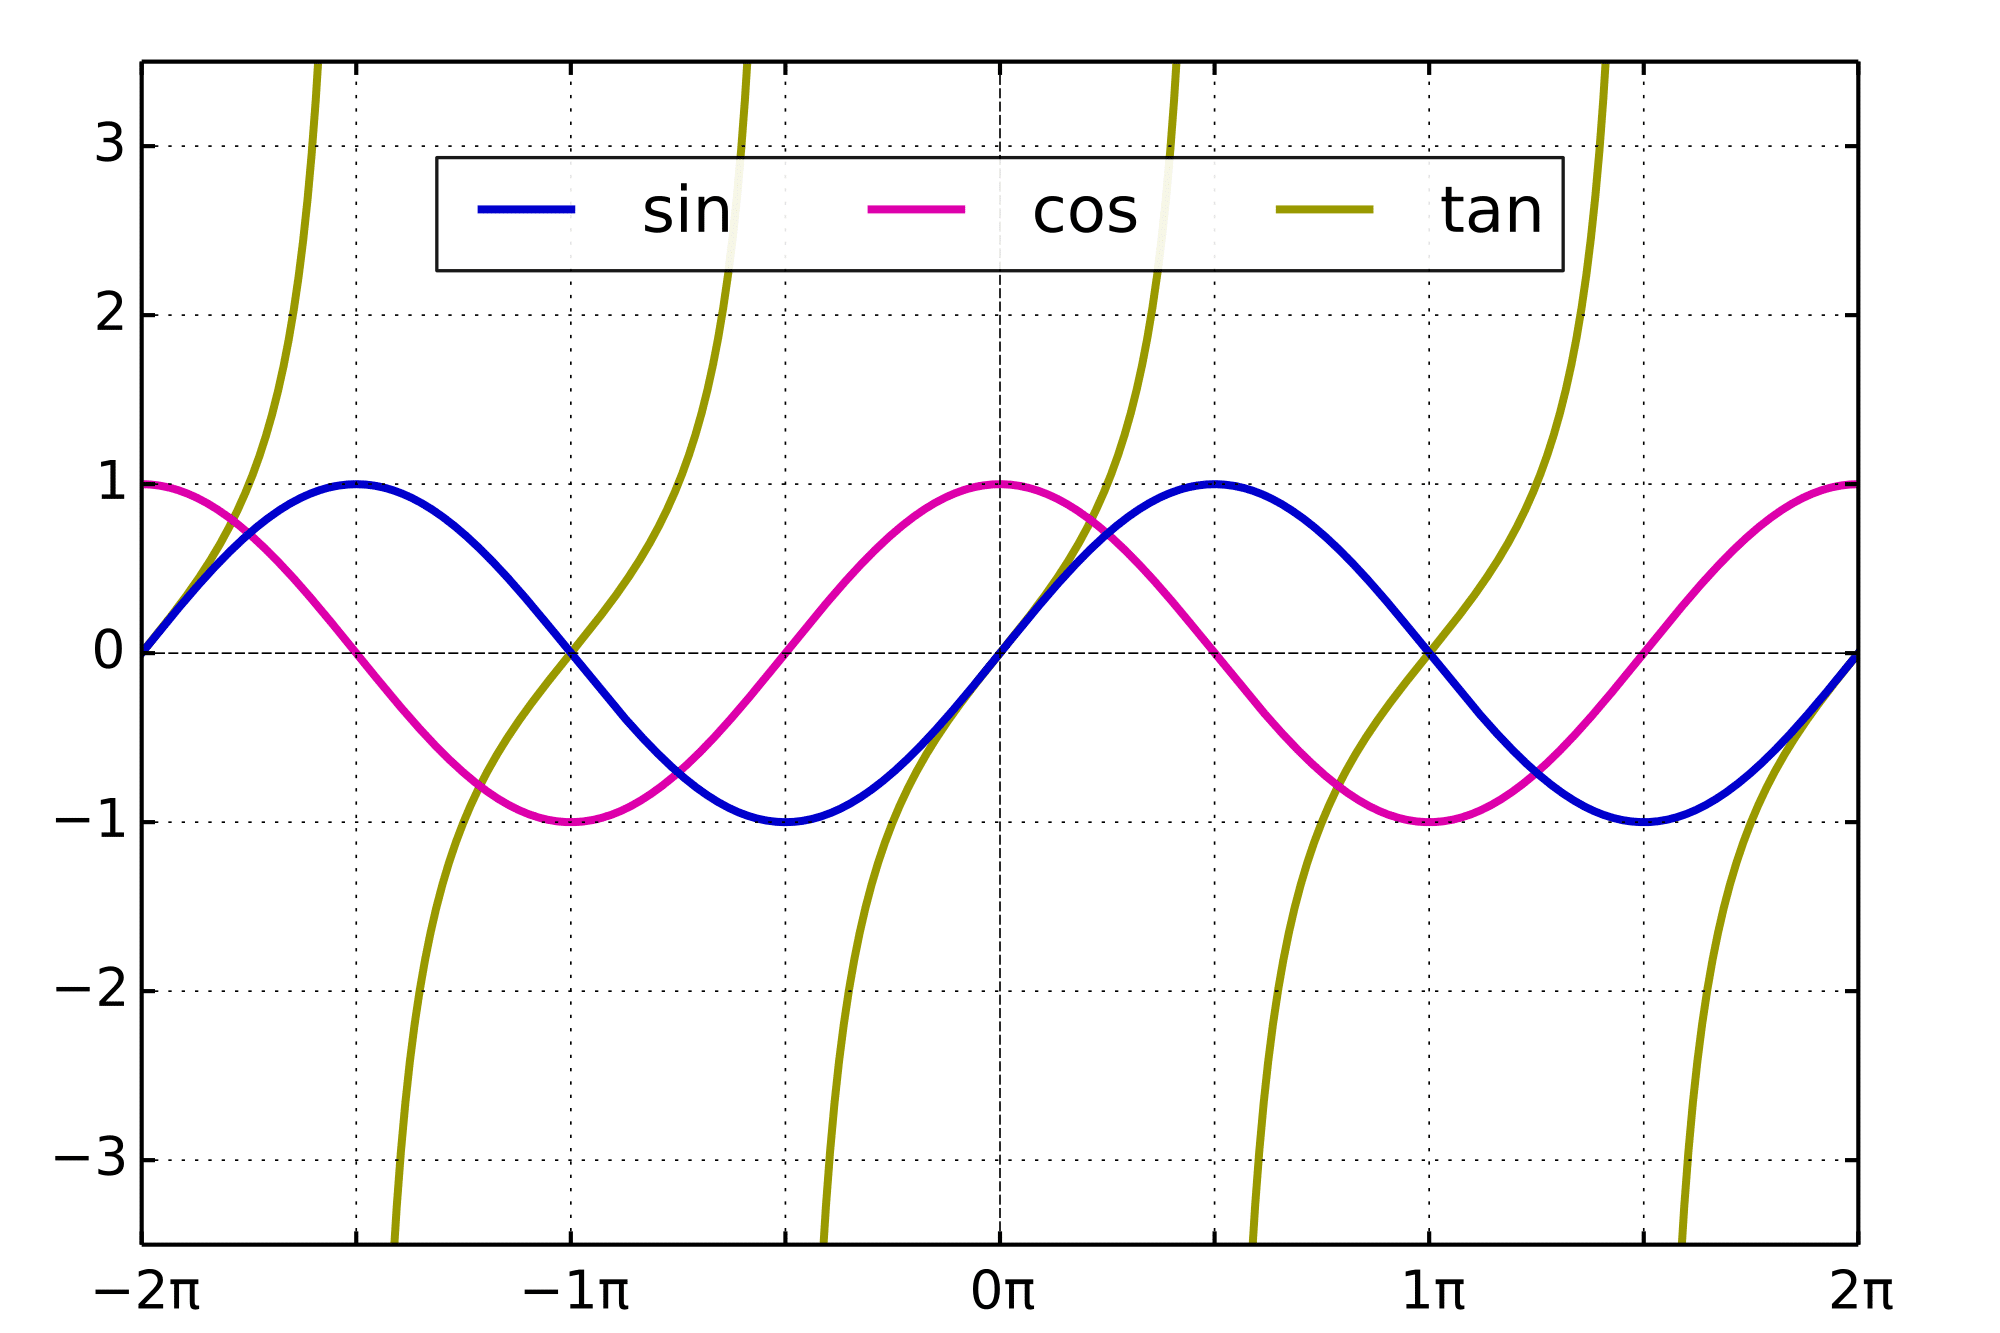
\includegraphics[width=5.5cm]{sincostan.png} \\
  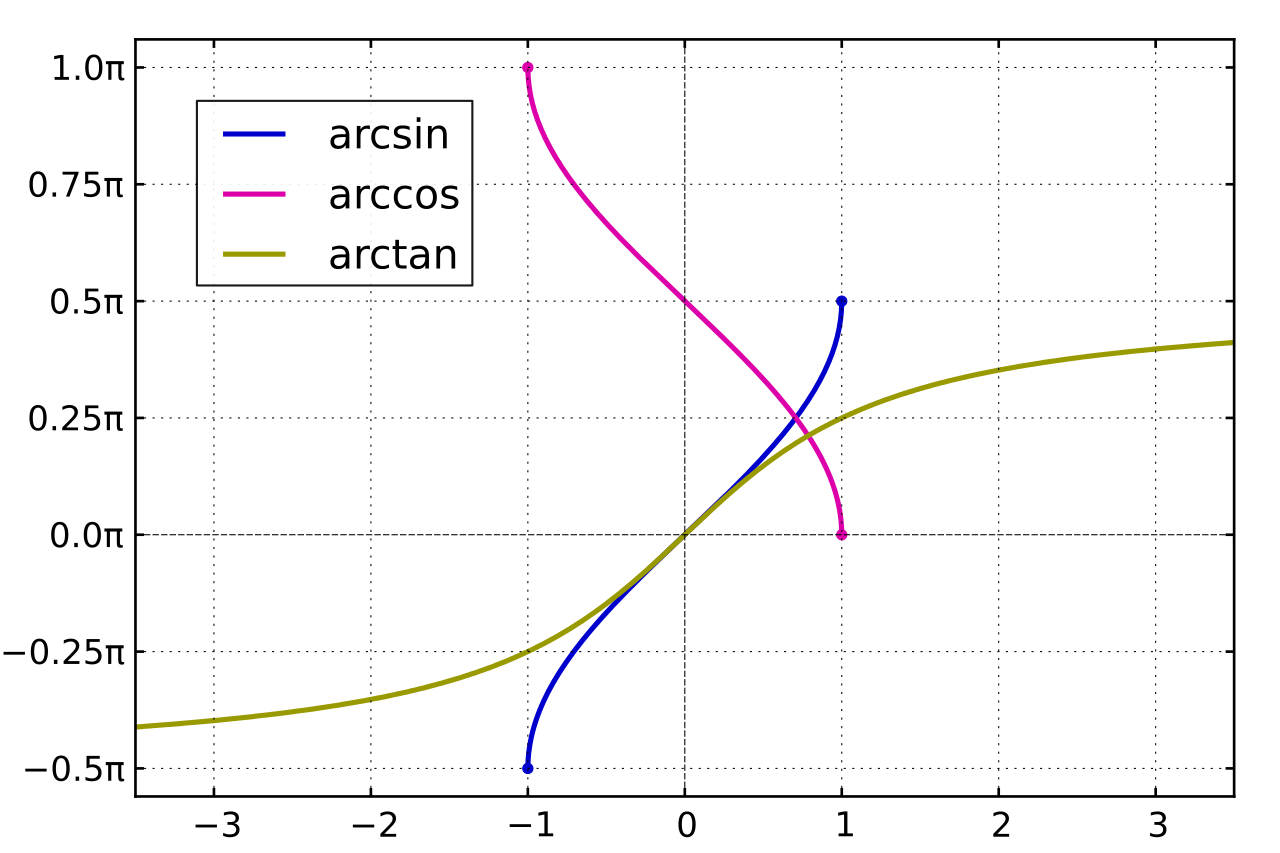
\includegraphics[width=5.5cm]{arcsinArccosArctan.png}\\
  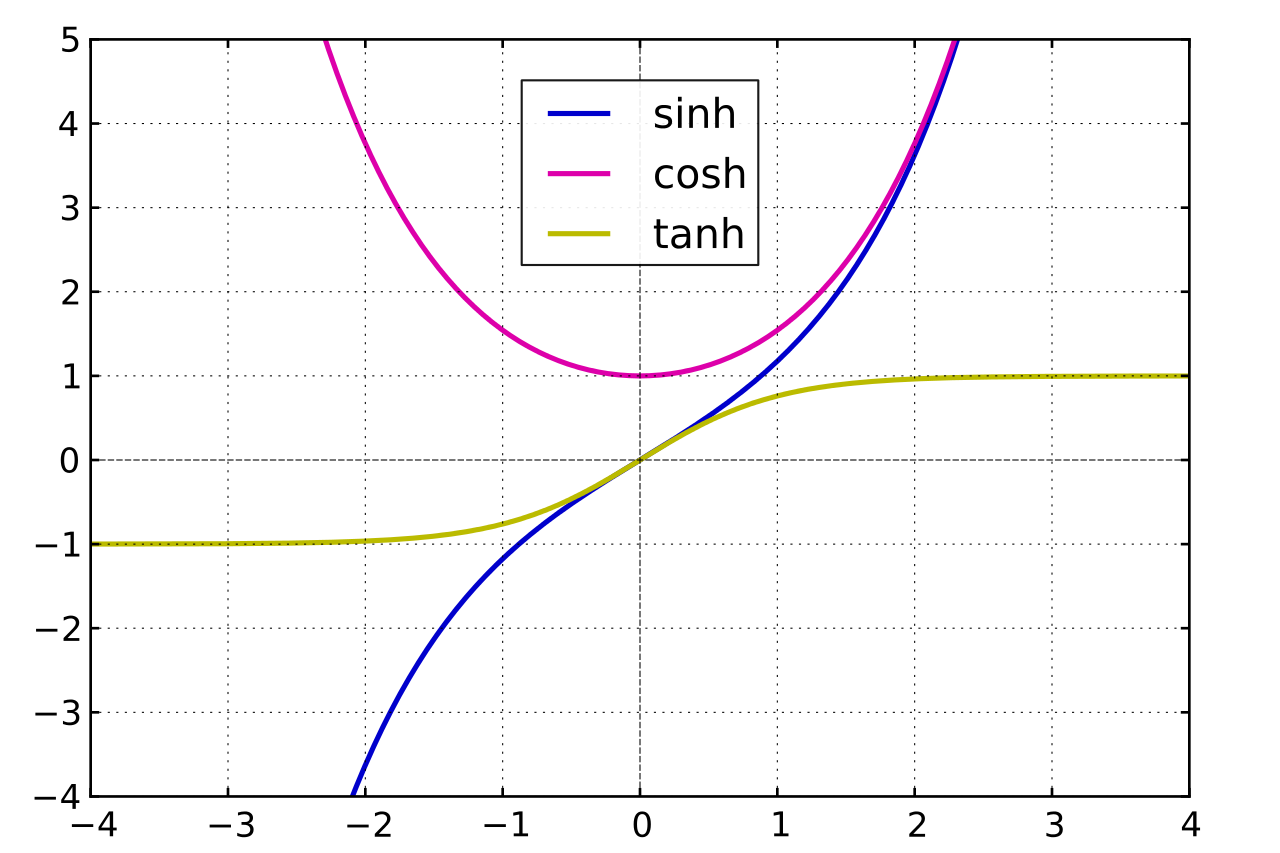
\includegraphics[width=5.5cm]{sinhCoshTanh.png}
  \end{center}

\section{Tabellen}
\subsection{Ableitungen}
\begin{center}
  \begin{tabularx}{\linewidth}{c>{\centering\arraybackslash}Xc}
  $\mathbf{F(x)}$ & $\mathbf{f(x)}$ & $\mathbf{f'(x)}$ \\
  %\midrule
  $(x-1)e^x $ & $xe^x$ & $(x+1)e^x$ \\ 
  $\frac{x^{-a+1}}{-a+1}$ & $\frac{1}{x^a}$ & $\frac{a}{x^{a+1}}$ \\
  $\frac{x^{a+1}}{a+1}$ & $x^a \ (a \ne -1)$ & $a \cdot x^{a-1}$ \\
  $\frac{1}{k \ln(a)}a^{kx}$ & $a^{kx}$ & $ka^{kx} \ln(a)$ \\
  $\ln |x|$ & $\frac{1}{x}$ & $-\frac{1}{x^2}$ \\
  $\frac{2}{3}x^{3/2}$ & $\sqrt{x}$ & $\frac{1}{2\sqrt{x}}$\\
  $-\cos(x)$ & $\sin(x)$ & $\cos(x)$ \\
  $ $ & $\frac{\sin(x)^2}{2} $ & $\sin(x)\cos(x)$ \\ 
  $\sin(x)$ & $\cos(x)$ & $-\sin(x)$ \\
  $\frac{1}{2}(x-\frac{1}{2}\sin(2x))$ & $\sin^2(x)$ & $2 \sin(x)\cos(x)$ \\
  $\tan(x) - x$ & $\tan(x)^2$ & $2\sec(x)^2 \tan(x)$\\
  $-\cot(x) - x$ & $\cot(x)^2$ & $-2 \cot(x) \csc(x)^2$\\
  $\frac{1}{2}(x + \frac{1}{2}\sin(2x))$ & $\cos^2(x)$ & $-2\sin(x)\cos(x)$ \\
  \multirow{2}*{$-\ln|\cos(x)|$} & \multirow{2}*{$\tan(x)$} & $\frac{1}{\cos^2(x)}$  \\
  & & $1 + \tan^2(x)$ \\
  $\cosh(x)$ & $\sinh(x)$ & $\cosh(x)$ \\
  $\log(\cosh(x))$ & $\tanh(x)$ & $\frac{1}{\cosh^2(x)}$ \\
  $\ln | \sin(x)|$ & $\cot(x)$ & $-\frac{1}{\sin^2(x)}$ \\
  $\frac{1}{c} \cdot e^{cx}$ & $e^{cx}$ & $c \cdot e^{cx}$ \\
  $x(\ln |x| - 1)$ & $\ln |x|$ & $\frac{1}{x}$ \\
  $\frac{1}{2}(\ln(x))^2$ & $\frac{\ln(x)}{x}$ & $\frac{1 - \ln(x)}{x^2}$ \\
  $\frac{x}{\ln(a)} (\ln|x| -1)$ & $\log_a |x|$ & $\frac{1}{\ln(a)x}$ \\

  %\bottomrule
  \end{tabularx}
\end{center}

%\subsection{Weitere Ableitungen}
\begin{center}
  \begin{tabularx}{\linewidth}{>{\centering\arraybackslash}X>{\centering\arraybackslash}X}
  
  $\mathbf{F(x)}$ & $\mathbf{f(x)}$ \\
  \midrule
  $\arcsin(x) / \arccos(x)$ & $\frac{1 / -1}{\sqrt{1 - x^2}}$ \\
  $\arctan(x)$ & $\frac{1}{1 + x^2}$ \\ 

  $x\arcsin(x) + \sqrt{1 - x^2}$ & $\arcsin(x)$\\
  $x\arccos(x) - \sqrt{1 - x^2}$ & $\arccos(x)$\\
  $x\arctan(x) - \frac{1}{2}\ln(1+x^2)$ & $\arctan(x)$\\
  $\ln(\cosh(x))$ & $\tanh(x)$\\

   
  $x^x \ (x > 0)$ & $x^x \cdot (1 + \ln{x})$ \\
$f(x)^{g(x)}$ & $e^{g(x) ln(f(x))}$\\
$f(x) = cos(\alpha)$ & $f(x)^n = sin(x + n\frac{\pi}{2})$\\
$f(x) = \frac{1}{ax + b}$ & $f(x)^n = (-1)^n * a^n * n! * (ax + b)^{-n+1}$\\
  $-\ln(\cos(x))$ & $\tan(x)$\\
  $\ln(\sin(x))$ & $\cot(x)$\\
  $\ln(\tan(\frac{x}{2}))$ & $\frac{1}{\sin(x))}$\\
  $\ln{(\tan(\frac{x}{2} + \frac{\pi}{4})}$ & $\frac{1}{cos(x)}$\\

  \bottomrule
  \end{tabularx}
\end{center}

    \subsubsection {Kritische Stelle}
  Eine \textbf{kritische Stelle} einer Funktion ist ein $x_0$ an der $f'(x_0)$ null
  oder undefiniert ist.
  % Hyperbol Funktionen

    \subsubsection {Hyperbol Funktionen}
  
  \begin{enumerate}[label=(\arabic*)]
    \item $cosh(x) := \frac{e^x + e^{-x}}{2}: \mathbf{R} \rightarrow [1, \infty]$
    \item $sinh(x) := \frac{e^x - e^{-x}}{2}: \mathbf{R} \rightarrow \mathbf{R}$
    \item $tanh(x) := \frac{e^x - e^{-x}}{e^x + e^{-x}}: \mathbf{R} \rightarrow [-1, 1]$
  \end{enumerate}
  und es gilt $cosh^2(x) - sinh^2(x) = 1$

%\subsection{Integrale}
\begin{center}
 \begin{tabularx}{\linewidth}{>{\centering\arraybackslash}X>{\centering\arraybackslash}X}
  
  $\mathbf{f(x)}$ & $\mathbf{F(x)}$ \\
  \midrule
  $\int f'(x) f(x) \dx$ & $\frac{1}{2}(f(x))^2$ \\
  $\int \frac{f'(x)}{f(x)} \dx$ & $\ln|f(x)|$ \\
  $\int_{-\infty}^\infty e^{-x^2} \dx$ & $\sqrt{\pi}$ \\
  $\int (ax+b)^n \dx$ & $\frac{1}{a(n+1)}(ax+b)^{n+1}$ \\
  $\int x(ax+b)^n \dx$ & $\frac{(ax+b)^{n+2}}{(n+2)a^2} - \frac{b(ax+b)^{n+1}}{(n+1)a^2}$ \\
  $\int (ax^p+b)^n x^{p-1} \dx$ & $\frac{(ax^p+b)^{n+1}}{ap(n+1)}$ \\
  $\int (ax^p + b)^{-1} x^{p-1} \dx$ & $\frac{1}{ap} \ln |ax^p + b|$ \\
  $\int \frac{ax+b}{cx+d} \dx$ & $\frac{ax}{c} - \frac{ad-bc}{c^2} \ln |cx +d|$ \\
  $\int \frac{1}{x^2+a^2} \dx$ & $\frac{1}{a} \arctan \frac{x}{a}$ \\
  $\int \frac{1}{x^2 - a^2} \dx$ & $\frac{1}{2a} \ln\left| \frac{x-a}{x+a} \right|$ \\
  $\int \sqrt{a^2+x^2} \dx $ & $\frac{x}{2}f(x) + \frac{a^2}{2}\ln(x+f(x))$ \\
  \bottomrule
 \end{tabularx}
\end{center}
  % Potenzen der Winkelfunktion

    \subsubsection {Potenzen der Winkelfunktion}
  
  $sin^2(x) = \frac{1}{2} (1 - cos(2x))$\\
  $cos^2(x) = \frac{1}{2} (1 + cos(2x))$\\
  \\
  % Funktionen Verknüpfung

    \subsubsection {Funktionen Verknüpfung}
  
  $
    x \mapsto (g \circ f)(x) := g(f(x))
  $\\ \\
  % Häufungspunkt

    \subsubsection {Häufungspunkt}
  
  $x_0 \in \mathbf{R}$ ist ein \textbf{Häufungspunkt} der Menge $\mathbf{D}$,
  falls $\forall \delta > 0 \;\;\; (]x_0 - \delta, x_0 + \delta[ \setminus \{x_0\}) \cap \mathbf{D} \neq \emptyset$\\ \\
  % Kritische Stelle

  %------------ Ordinary differential equations (ODE's) ---------------
  \subsection{Ordinary differential equations (ODE's)}
  Given $F$, a function of $x, y$, and derivatives of y.
  Then an equation of the form
  \begin{align*}
    F(x, y, y', \dots, y^{(n)}) = 0
  \end{align*}
  is an implicit ODE of order $n$. Order is determined
  by the highest derivative. Implicit means the
  equation equals $0$.

  %------------ Homogenous ---------------
\subsection{Homogenous}
A linear ODE is homogenous when $b(x) = 0$.
Inhomogenous otherwise.
\end{multicols*}
\end{document}